%!TEX ROOT=../ctutest.tex

\chapter{State of the Art}
%--- FIG: UTF forms

This chapter will first describe the originally popular models for general NLP, such as BERT and the recent paradigm shift from \textit{pretrain + finetune} transfer learning framework popular since the original~\cite{devlin2019bert} paper to the currently booming LLMs, which often outperform the smaller models even without the fine-tuning step~\cite{gpt4, llama, vicuna}. We will then take a look at the performance optimization methods that enable training multi-billion parameter pre-trained models on a set of task-specific data on a single GPU and their potential for our research. 

To show how it relates to our main topics, we will introduce currently published approaches for the automated fact-checking task, efforts related to claim generation, and evaluation of NLP model outputs.

\label{chap:sota}
\section{Pretrain + Finetune}
\label{sec:pretrain}
For the last decade, the \textit{pretrain-finetune} paradigm has been a cornerstone in Natural Language Processing (NLP). It has significantly shaped the development of modern NLP models. Its use in NLP can be traced back to the advent of neural networks and deep learning in the early 2010s. Initially, researchers pre-trained word embeddings using methods like Word2Vec~\cite{mikolov} and GloVe~\cite{pennington-etal-2014-glove}, which captured semantic relationships among words and then tweaked the general-task models for various related tasks.

\subsection{BERT and derivatives}\label{sec:bert}
The \textit{pretrain-finetune} paradigm truly rose to fame with the introduction of transformer-based models, particularly the revolutionary BERT (Bidirectional Encoder Representations from Transformers) in 2018. BERT~\cite{devlin2019bert} demonstrated the power of pretraining large-scale language models on massive text corpora using an easy-to-automate general task such as \textit{Masked Language Modeling}, or \textit{Next Sentence Prediction}, followed by fine-tuning on specific downstream tasks using smaller, harder-to-obtain data. This approach achieved state-of-the-art results across various NLP benchmarks. Subsequently, numerous variations of pre-trained models like GPT (Generative Pre-trained Transformer) and RoBERTa emerged, each refining the pretrain-finetune paradigm to improve language understanding, generation, and transfer learning capabilities. 

Importantly, BERT's success inspired many publications in training similar transformer models, varying in the definition of the general pre-training task, model size, architecture training corpus

\begin{itemize}
    \item In Czech language, monolingual models CZERT~\cite{czert}, FERNET~\cite{fernet}, RobeCzech~\cite{straka2021robeczech}, and small-e-czech~\cite{kocian2021siamese} are available for further finetuning
    \item In Polish, HerBERT~\cite{mroczkowski-etal-2021-herbert} achieved state-of-the-art in multiple tasks in 2021
    \item In Slovak, SlovakBERT~\cite{pikuliak2021slovakbert} was released by KInIT and Gerulata
    \item A multitude of multilingual models, such as \MBERT or \XLM~\cite{xlm-roberta} were pre-trained on data in all three of these languages (and many others), proving that the large transformers can capture a notion of semantics and relations between pieces of text even \textit{without} the convenient constriction of a single language 
\end{itemize}

\section{Few-shot and Zero-shot learning}
\label{sec:llms}
The ever-growing (sometimes billions of parameters in size) transformer models have not only demonstrated superior performance on benchmark datasets but have also shown remarkable zero-shot and few-shot learning abilities, where they can perform tasks with minimal or no task-specific training data~\cite{gpt3}.

Few-shot learning refers to the capability of a model to perform a task when provided with only a limited amount of labeled examples. Zero-shot learning takes this concept a step further by enabling models to tackle tasks they have never seen during training. The integration of these learning paradigms into large language models like GPT-3 and subsequent iterations has spread the NLP hype even further. By utilizing a prompt or a few examples, these models can quickly adapt to new tasks, making them highly versatile, adaptable, and usable to the general public.
\subsection{OpenAI LLMs: GPT-3 and GPT-4}
\label{sec:gpt}
In 2020, the few-shot learning was exhibited on GPT3 -- a 175B-parameter autoregressive model trained by~\cite{gpt3}. The model was trained on the task of generating text based on user's and its own previous outputs.
The training procedure and data\footnote{A mixture of crawled websites, books, and Wikipedia.} is thoroughly described in the publication. However, it is prohibitively costly for most labs to reproduce or even fine-tune at such a scale. 

In the fall of 2022, GPT-3 became widely popular thanks to its \textsf{ChatGPT}\footnote{\url{https://chat.openai.com}} fine-tune and demonstration app, which puts the user in the role of \textit{prompter}, texting back and forth with an LLM that predicts the most fitting reply to each conversation.

With the arrival of GPT-4, the \textsf{ChatGPT} was already massively famous, and the new model already shipped with a paid-service business scheme no longer publishing the training data, tasks, or even model size~\cite{gpt4}.

\section{Open source LLMs}
This puts the research community in an awkward position, as the GPT-4 achieves state-of-the-art in numerous NLP benchmarks~\cite{gpt4, Liu_2023}, but is designed not to be used in any way other than as a black box, making the derived research rigorosity and reproducibility disputable.

From the prediction times, \textsf{OpenAI} claims, and general trends in NLP, there are also reasons to believe that GPT-4 is orders of magnitude larger than already wasteful GPT-3.
This motivates an uptick in research of other LLMs that would be able to operate on a smaller scale with similar results, using a peer-reviewed architecture, training scheme, and data that is available in open source.

\subsection{LLaMA-2 and derivatives}
\label{sec:llama}

A popular foundational LLM to compete with the GPT family has become the \textsf{LLaMA}~\cite{llama} from \textsf{Meta research}. LLaMA was trained on about 5TB of publicly available textual data\footnote{To be specific, LLaMA was trained using an autoregressive language modeling task on a mixture of English CommonCrawl Corpus, C4~\cite{raffel2020exploring}, Github, Wikipedia, Gutenberg Project, Books3 corpus, ArXiv and Stack Exchange} mainly in English. 

It comes in various sizes between 7B and 65B parameters, achieving a SOTA among open-source solvers in various tasks and an unmatched performance in the field of single-GPU (7B and 13B) model sizes.
LLaMA proceeds to be used as a goto base model for a number of successful open-source chatbots such as Alpaca~\cite{alpaca}, Vicuna~\cite{vicuna}, and OpenAssistant~\cite{openassistant}.

The pre-trained LLaMA weights are, however, published under a restrictive license that prohibits republishing the model weights even after tuning its parameters, which limits its fine-tuners to publishing delta- or xor-weights that can not be properly used without \textsf{Meta}'s permission.

LLaMA-2~\cite{llama2} addresses this inconvenience (as well as delivers its own take on the \textit{chatbot} task), yielding an ideal strong base model for experimentation with any NLP task in 7B, 13B, and 70B sizes.
The only obstacle left in the way is the computational cost of fine-tuning across so many parameters.

%Open-source, freely usable.
%Often poor czech coverage 
%Quantizace, 4b, 8b, zlomek parametrů\cite{openassistant}

\subsection{LoRA and other optimization}\label{sec:lora}
To be able to fine-tune multi-billion-parameter models such as \textsf{LLaMA-2}~\cite{llama2} on a single TPU, successful approaches have been published to dramatically cut down the training expenses.
Parameter-efficient fine-tuning (PEFT)~\cite{peft} proposes approaches to only fine-tune \textit{a few} weights as opposed to the whole neural network, reducing the number of trainable parameters by orders of magnitude.
Low-Rank Adaptation of Large Language Models (LoRA)~\cite{lora} does so by freezing the pre-trained model weights and injecting trainable rank decomposition matrices into each layer of Transformer architecture. 

Quantization, which cuts the costs of working with 32- or 16-bit float parameters and opting for data types of bitsize as small as 4, also proves to be a powerful tool for LLM finetuning performance optimization~\cite{dettmers2023qlora}.
Quantized QLoRA takes LLaMA and finetunes it into a Guanaco model family, which outperforms all previous openly released LLMs on Vicuna benchmark~\cite{dettmers2023qlora} and achieves 99.3\% of the ChatGPT's performance on it while only requiring 24 hours on a single GPU.

As per an alleged leaked Google memo~\cite{moat}, this could put the future state of the art in NLP disciplines back into the hands of open source and public research, not giving any of the big tech companies a \"{moat} advantage.

Either way, it goes to show that the open-source LLMs have a promising future in NLP and will be indismissible as an approach for the NLP task of \textit{Automated fact checking}.

\section{Fact checking approaches}
Back in the late 2010s, the misinformation and its spread in the era of the internet and social media became a discussed topic in the Western world, with multiple institutions such as the European Council marking it a severe threat to democracy and national safety~\cite{disorder}.
The public attention and maturation of appropriate technologies motivated numerous efforts in business and academia to tackle the challenge.
Among other events, a Fake News Challenge occurred in 2017~\cite{fncweb} exploring the uses of technologies in the field and applying, for example, the LSTMs to detect stances among textual data~\cite{fnc}.

\subsection{FEVER and followups}
Soon, standard tasks began to be formulated and data collected. 
The FEVER (Fact Extraction and VERification)~\cite{fever} dataset and shared task became prominent in natural language processing research.
Relatively early on, it formalized the task as a two-step problem:
\begin{enumerate}
    \item Retrieving information within a structured corpus to fact-check a given claim (this resembles a standard NLP problem called \textit{information retrieval} -- IR)
    \item Classifying the inference relation between retrieved information and claim as one of:
    \begin{enumerate}
        \item {\techbf supports} -- information semantically implies the claim 
        \item {\techbf refutes} -- information semantically implies the negation of the claim 
        \item {\techbf not enough info} otherwise 
    \end{enumerate}
    This classification task became known as \textit{natural language inference} and mostly replaced the previous binary classification NLP task of \textit{recognizing textual entailment} (RTE)
\end{enumerate}

The FEVER dataset was a collection of 185K human-annotated claims, their veracity labels, and sets of evidence from a structured corpus that sufficed to justify the labels.
The corpus of choice was a 2017 English Wikipedia structured into articles due to its reasonable size, informational richness, and open license.\footnote{Is Wikipedia a trustworthy informational canon, though? 
No, it is not supposed to -- FEVER states that it is crucial to always maintain that the fact-checking classifiers only classify \textit{with respect to} data, and their reliability goes only as far as that of the underlying knowledge corpus. Therefore, \textit{supports} does not directly translate to \textit{true}, nor \textit{refutes} to \textit{false}}

FEVER yields an interesting benchmark with statistically quantifiable model success, motivated multiple well-performing public solutions~\cite{fever1,fever2}, gives insights into the complexities of automated fact-checking task, and strong baselines for research in the field. The data was later enriched by contrastive evidence in VitaminC~\cite{DBLP:journals/corr/abs-2103-08541} and by reasoning over tabular data in FEVEROUS~\cite{aly2021feverous}.

To date, it keeps being a reference point in automated fact-checking research despite its limitations, such as its requirement for a fixed knowledge base and \"{atomicity}\footnote{See section 4.1.2.\ref{atomicity}} of claims.

\begin{figure}
    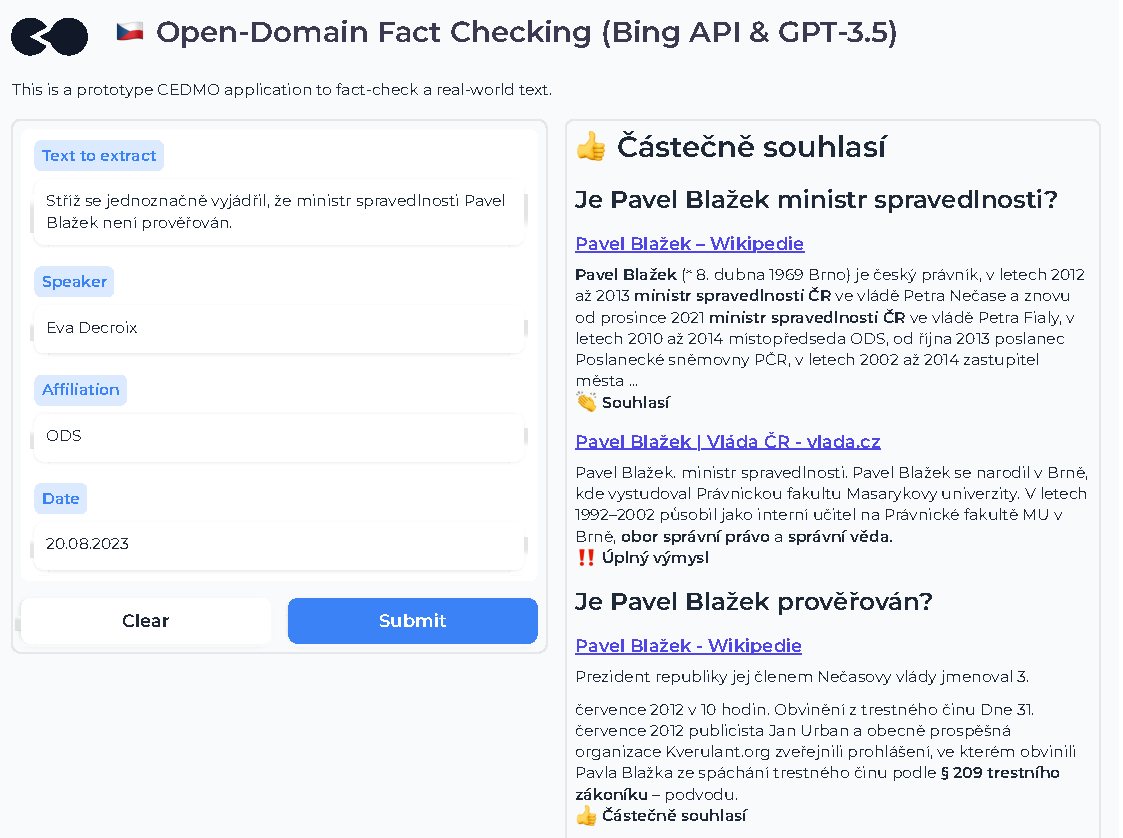
\includegraphics[width=14cm]{fig/bing.pdf}
    \caption{Proof-of-concept Czech fact-checking based on live-internet search (Bing API) and LLM prompting, based on the proposals of~\cite{bing} in Czech, using a real-world claim that was fact-checked by \href{https://demagog.cz/vyrok/22849}{\url{demagog.cz}} in June 2023}
    \label{fig:bing}
\end{figure}

\subsection{Open-domain fact-checking}
Due to these limitations, some researchers consider the scheme from FEVER an oversimplification -- the real politics' claims to be fact-checked by journalists often consist of long syntactical structures, combine information together in a non-trivial manner and often require the most up-to-date evidence. 

\"{Complex Claim Verification with Evidence Retrieved in the Wild}~\cite{bing} proposes a different scheme that overcomes these shortcomings:

\begin{enumerate}
    \item Arbitrarily complex claim is decomposed into a set of yes/no questions
    \item An open-domain search (Bing is proposed in the paper) fetches several evidence documents for each question
    \item A claim-focused summary is extracted from each document
    \item A veracity classifier goes through each pair of evidence and question, ranging from \"{faithful} to \"{completely wrong}
    \item The scores are combined (all need to be \"{faithful} for a faithful claim. Otherwise, the severity of inaccuracies can be approximated using some averaging.
\end{enumerate}

GPT-3 is used in steps 1, 3, and 4 of the scheme in the prototype delivered in~\cite{bing} in a few- and zero-shot fashion, with few-shot unsurprisingly coming out a little better. The scheme is transducible to Czech, and Figure~\ref{fig:bing} shows my early experiments with my interactive reproduction of it, predictors based on Bing and GPT-3.5 (a polished version of GPT-3).

While the shift from an established FEVER framework to complex real-world claims and evidence retrieval \"{in the wild} feels exciting and practical, an obvious pitfall arises -- anyone can publish anything on the internet, having it appear in Bing search and other crawlers alike. I argue that this might lead into a sort of a circular dependency of needing to reliably fact-check the evidence we have retrieved from the web in order to be able to build a reliable fact-checker in the first place.

Anyhow, the open-domain fact-checking idea opens a whole new range of approaches and shows the power of LLMs in fact-checking at its every step.

\section{Claim generation}
Another step of the fact-checking pipeline, covered by very few research publications, is the generation of the claim to be checked in the first place~\cite{guo-etal-2022-survey}.

The current state of things is that journalists who fact-check statements within, say, a Facebook status, need to read through the whole document multiple times, formulate its factual claims from the stances and facts expressed in the text themselves, and then fact-check each separately.

What has been examined so far were, for example:
\begin{itemize}
    \item Using Question Generation (QG) solver and converting the questions into declarative sentences to emulate more claims and more data for fact checking~\cite{pan2021zeroshot}
    \item Numerous CLEF CheckThat! challenges explored the task of estimating \textit{checkworthiness} of different parts of a long text, such as lines in a political debate~\cite{clef19,clef21}
    \item The task of extreme summarization (XSum) consists of summarizing a long body of text into a single sentence, focusing on its most relevant aspects and facts. Large datasets XSum~\cite{narayan-etal-2018-dont} in English and XL-Sum~\cite{xlsum} in 44 languages both present expertly annotated data from BBC News for it, as their article standard features a single-sentence summary at the beginning of each text.
\end{itemize}

\subsection{NLP summarization benchmarking}
\label{benchmarking-sota}
An important caveat to note with the NLP tasks reducing longer text to shorter text -- such as summarization or claim extraction -- is that the standard automatic metrics such as ROUGE~\cite{lin-2004-rouge} and METEOR~\cite{banerjee-lavie-2005-meteor} only focus on the \textit{content selection} aspect of tasks, based on a word-by-word overlap and were designed to use on multiple gold summaries per input, which are not often provided with modern large-scale datasets.~\cite{nlpprogress,bert-score,zha2023alignscore}

These serious limitations make it questionable for anyone to claim state-of-the-art on these tasks and motivate research for new metrics to cover all the important aspects of claim generation and do so in correlation with expert human judgment. 

This will be the topic of section~\ref{metrics}, which also introduces the state-of-the-art research we are working with to arrive to a valid set of benchmarks.